\documentclass[10pt,conference,letterpaper]{IEEEtran}
\usepackage{times,amsmath,epsfig}
\usepackage{enumerate,cite,url}

\title{RiskFinder: A Sentence-level Financial Risk Detector for Financial Reports}
\author{
{Yu-Wen Liu{\small $~^{\#1}$}, Liang-Chih Liu{\small $~^{*2}$}, Chuan-Ju Wang{\small $~^{\#3}$}, Ming-Feng Tsai{\small $~^{\&4}$} }

\vspace{1.6mm}\\
\fontsize{10}{10}\selectfont\itshape
$^{\#}$\,Department of Computer Science, National Chengchi University\\
%Address Including Country Name\\
\fontsize{9}{9}\selectfont\ttfamily\upshape
\{{$^{1}$g10435,$^{4}$mftsai\}}@cs.nccu.edu.tw\\
%$^{4}$\,@cs.nccu.edu.tw

%\vspace{1.2mm}\\
\fontsize{10}{10}\selectfont\rmfamily\itshape
$^{*}$\,Department of Information and Finance Management, National Taipei University of Technology\\
%Address Including Country Name\\
\fontsize{9}{9}\selectfont\ttfamily\upshape
$^{2}$\,lcliu@ntut.edu.tw\\

\fontsize{10}{10}\selectfont\rmfamily\itshape
$^{*}$\,Research Center of Information Technology Innovation, Academia Sinica\\
%Address Including Country Name\\
\fontsize{9}{9}\selectfont\ttfamily\upshape
$^{3}$\,cjwang@citi.sinica.edu.tw\\
}

\begin{document}
\maketitle
\begin{abstract}
    This paper demonstrates RiskFinder, a web-based information system for facilitating the analyses of soft and hard information in financial reports. In particular, the system broadens analysis from the word level to the sentence level; this is novel in practitioner communities and unprecedented among financial academics. The proposed system has four main components: 1) a Form 10-K risk-sentiment dataset, consisting of a set of labeled financial sentences and pre-trained sentence embeddings; 2) metadata, including basic information on each company that published the Form 10-K financial report as well as some relevant financial measures; 3) an interface that highlights risk-related sentences in the financial reports based on several sentence embedding techniques; 4) a visualization of financial time-series data for the corresponding company.
    %This system considerably facilitates case studies in the field of finance and can be of great help in capturing valuable insight within large amounts of textual information.
    This system can be of great help in capturing valuable insight within large amounts of textual information.

\end{abstract}

\section{Introduction}
    A great deal of mass media outlets such as newspapers and magazines, or financial report disclosures required by authorities such as the SEC\footnote{SEC indicates Securities and Exchange Commission}-mandated Form-10Q and Form-10K, play an important role in disseminating information to participants in financial markets. The spread of this information may quickly or slowly influence the sentiment of market participants and thus reshape their perspectives on economic numbers, such as stock prices and interest rate levels. This information comes in two types: soft information, usually referring to textual information such as opinions, ideas, and market commentary; and hard information, that is, numerical information such as historical time series of stock prices.

    Due to the strong relation between the textual information and numerical measures, there have been a growing body of studies in the fields of finance and data science that adopt the techniques of natural language processing (NLP) and machine learning to examine the interaction between these two types of information~e.g.\cite{kogan2009predicting,tsai2017risk,Tsai:2016:DFK:2991040.2948072,rekabsaz2017volatility}. For example, these studies~\cite{loughran2011liability,jegadeesh2013word} investigate how the disclosures of finance sentiment or risk keywords in SEC-mandated financial reports affect investor expectations about a company's future stock prices. Moreover, several studies~\cite{kogan2009predicting,tsai2017risk} exploit sentiment analysis of 10-K filing reports for financial risk analysis. Furthermore, in~\cite{liu2016fin10k} a web-based information system, \textsc{Fin10K}, is proposed for financial report analysis and visualization. However, these studies and systems all focus on word-level analysis, which likely yields biased results because most financial keywords are context-sensitive~\cite{liu2016fin10k}. Therefore, to advance the understanding of financial textual information, this paper further constructs an information system based on sentence-level analysis to assist practitioners to capture more precise and meaningful insight within large amounts of textual information in finance.

    In NLP, several research studies have been conducted to produce a distributed representation of words, such as word2vec~\cite{Mikolov:2013:DRW:2999792.2999959}. Most word embedding techniques rely on a neural network architecture instead of the more traditional $n$-gram models and unsupervised learning; this is because neural networks have a rather remarkable ability to turn meaning into numbers. In addition, there have also been some extensions of word embeddings for sentences, paragraphs, or even documents, such as doc2vec~\cite{Mikolov:2013:DRW:2999792.2999959}, FastText~\cite{bojanowski2016enriching}, and Siamese-CBOW~\cite{kenter2016siamese}.

    Following the fruitful progress of these techniques of word and sentence embeddings, this paper presents RiskFinder, a web-based information system that broadens the content analysis from the word level to the sentence level for financial reports on Form-10K. The system has four main parts: 1) a Form 10-K risk-sentiment dataset, consisting of a set of labeled  financial sentences and pre-trained sentence embeddings; 2) metadata that summarizes the basic information about each financial report; 3) an interface that highlights risk-related sentences in the financial reports; 4) a visualization of financial time-series data associated with the corresponding financial reports. The proposed system, RiskFinder, is built on the 10-K Corpus~\cite{liu2016fin10k}, which contains 40,708 financial reports from year 1996 to 2013. In addition to the original 10-K corpus, we construct a set of labeled financial sentences with respect to financial risk by involving 8 financial specialists including accountants and financial analysts to ensure the quality of the labeling. With the labeled sentences and the large collection of financial reports, we apply FastText~\cite{bojanowski2016enriching} and Siamese-CBOW~\cite{kenter2016siamese} to sentence-level textual analysis. The system then automatically highlights risk-related sentences in those reports and categorizes these sentences as being positively, negatively, or insignificantly related to financial risk. For comparison purposes, the numbers of high-risk and low-risk sentences are summarized for the selected report, and we at the same time display the time-aligned relevant quantitative information such as the historical stock prices of the selected company to visualize its financial risk, which considerably facilitates case studies in the field of finance and accounting. Finally, we publish the pre-trained sentence vectors trained on the 10-K corpus and our constructed labeled sentences.

\section{System Description}\label{sec:system}
\begin{figure*}
  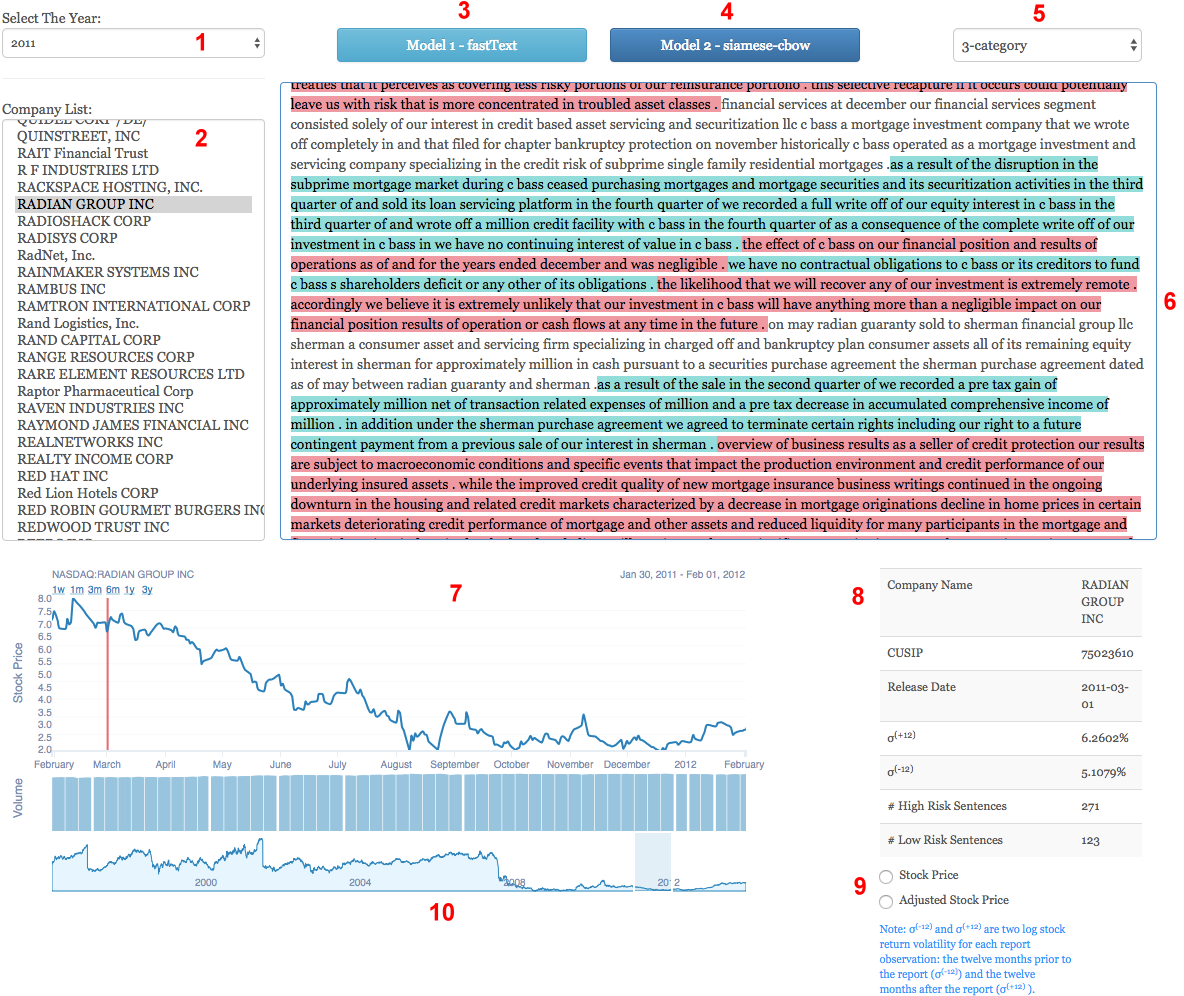
\includegraphics[width=6.6in]{fig/platformdescription.png}
  \caption{The user interface of the RiskFinder system}\label{fig:platformdescription}
\end{figure*}
Figure~\ref{fig:platformdescription} shows the user interface of the proposed RiskFinder system. In the system, there are 4 major components for risk detection, the details of which are provided in the following subsections.

\subsection{Form 10-K Risk-sentiment Dataset}
    The first component is the collection of the Form 10-K risk-sentiment dataset. This work provides the financial risk-sentiment dataset that consists of two types of data: a set of labeled financial sentences and the pre-trained sentence embeddings. There are in total 432 labeled financial sentences in the dataset, which were selected from the MD\&A\footnote{Management Discussion and Analysis of Financial Condition and Results of Operations} sections of the 10-K corpus. When selecting the candidate sentences, we first used the six financial sentiment lexicons proposed by~\cite{loughran2011liability} to filter sentences and randomly chose 24 sentences for annotation per year, yielding in total 432 sentences for 18 years (1996 to 2013). To construct the risk-labeled dataset, eight financial specialists including accountants, financial analysts and consultants participated in the annotation task to ensure the quality of the labeling. In the annotation process, each of the candidate sentences was labeled by three different annotators, and then the rule of majority was used to determine the degree of risk of the sentence. Cronbach's alpha which is regarding as an indicator to determine the internal consistency showed the reliability of 0.784. Table~\ref{tab:labelsummary} summarizes the annotation results.  In addition, the dataset also includes the pre-trained sentence vectors, each of which is a 100-dimension real-valued vector, trained by FastText and Siamese-CBOW on the 10-K corpus and the labeled sentences.\footnote{The dataset is available at \url{https://clip.csie.org/RiskFinder/} upon publication.}

\begin{table}[ht]
\centering
    \caption{Labeled sentences}
    \label{tab:labelsummary}
    \begin{tabular}{|c|c|c|c|c|}
        \hline
        mDegree of risk & High risk & Neutral & Low risk & Total\\
        \hline
        \# of sentences - training & 109 & 199 & 37 & 345\\
        \hline
        \# of sentences - testing & 29 & 29 & 29 & 87\\
        \hline
    \end{tabular}
\end{table}

\subsection{The Metadata}
    The second component of the proposed system is the metadata of the companies in the Form 10-K corpus, including basic information on each company such as the financial report and several financial measures. A user can first select the year from 1996 to 2013 of the financial reports in the selection bar (1) of Figure~\ref{fig:platformdescription} and pick the company documenting the report in that year in the list (2) (e.g., RADIAN GROUP INC in the figure). Following the selection, the MD\&A section of the chosen report\footnote{Only Section 7 MD\&A is used because it contains the most important forward-looking statements about the company and is thus related to future financial risk~\cite{kogan2009predicting,loughran2011liability}.} is then automatically loaded in the window (6). Then, our system simultaneously displays in table (8) the following metadata which summarizes the basic information of the corresponding company:

\begin{enumerate}[(a)]
  \item the company name;
  \item the company's CUSIP number, which facilitates the retrieval of information associated with this company from other widely used databases (e.g., Compustat and CRSP\footnote{CRSP is the abbreviation for the Center for Research in Security Prices.});
  \item the report release date;
  \item the annualized stock return volatilities measured in the twelve-month period before and after the announcement of the report (i.e., $\sigma^{(-12)}$ and $\sigma^{(+12)}$);
  \item the number of highlighted risk-related sentences in this report.
\end{enumerate}

\subsection{Risk-related Sentence Detection}
\begin{table*}[ht]
    \centering
    \caption{Performance for risk sentence classification}\label{tab:precision}
    \begin{tabular}{|l|c|c|c|c|c|c|c|c|c|c|}
        \hline
        & \multicolumn{4}{c|}{Binary classification} & \multicolumn{6}{c|}{Three-class classification}\\
        \cline{2-11}
         & \multicolumn{2}{c|}{Siamese-CBOW} & \multicolumn{2}{c|}{FastText} & \multicolumn{3}{c|}{Siamese-CBOW} & \multicolumn{3}{c|}{FastText}\\
        \hline
        Accuracy & \multicolumn{2}{c|}{0.656} & \multicolumn{2}{c|}{0.813} & \multicolumn{3}{c|}{0.503} & \multicolumn{3}{c|}{0.514} \\
        \cline{2-11}
        & High risk & Low risk  & High risk & Low risk  & High risk & Neutral  & Low risk & High risk & Neutral & Low risk  \\
        \hline
        Precision & 0.776 & 0.603 & 0.774 & 0.828 & 0.620 & 0.445 & 0.336 & 0.778 & 0.609 & 0.867 \\
        \hline
        Recall & 0.438 & 0.872 & 0.621 & 0.905 & 0.578 & 0.802 & 0.112 & 0.879 & 0.853 & 0.405 \\
        \hline
        F1-measure& 0.558 & 0.713 & 0.684 & 0.864 & 0.597 & 0.572 & 0.167 & 0.825 & 0.710 & 0.550 \\
        \hline
    \end{tabular}
\end{table*}

    To gauge a company's financial risk given the textual information in its financial reports on Form 10-K, the proposed system focuses on the sentence-level investigation into the MD\&A section, which is considered the part where the firm managements are most likely to reveal information by the tone they use~\cite{loughran2011liability}. In our system, two sentence embedding techniques are utilized for sentence-level textual analyses: Model 1 is FastText which uses a linear classifier that enables efficient sentence classification and yields performance on par with other deep learning classifiers~\cite{bojanowski2016enriching}; Model 2 is Siamese-CBOW, an efficient neural network architecture that obtains high-quality word embeddings, directly optimized for sentence representations~\cite{kenter2016siamese}. Since Siamese-CBOW, the second approach, produces only sentence embedding (by simply averaging the word embedding of each word in a sentence), we then employ a logistic regression to construct a classifier.

    As shown in Figure~\ref{fig:platformdescription}, by clicking button (3) or (4), users use Model 1 or 2 to classify the sentences in the MD\&A section for a certain financial report into three parts: those highlighted red representing high-risk sentences; those highlighted green representing low-risk ones; and others representing those irrelevant to financial risk. The three-class classification task can be reduced to a binary one through the selection bar (5): high-risk sentences in red and others in white. Table~\ref{tab:precision} tabulates the performance of both classification tasks tested on the 87 sentences in terms of accuracy, precision, recall, and F1-measure with 4-fold cross-validation.\footnote{The 432 sentences are split into the training data and the testing data with 345 and 87 sentences, respectively, and we use logistic regression as the classifier.} Note that for binary classification, we consider both neutral and low-risk sentences as irrelevant to financial risk. Finally, the numbers of highlighted risk-related sentences are summarized in table (8) of Figure~\ref{fig:platformdescription}.

\subsection{Visualization for Financial Measures}
    Our system attempts to facilitate the analysis of textual information and capture more insight into the financial risk associated with the announcement of each financial report. Therefore, in addition to highlighting the risk-related sentences, our system also displays time-aligned quantitative information for comparison purposes, such as historical prices and trading volumes of the selected company's stock, as shown in the chart (7) of Figure~\ref{fig:platformdescription}. In particular, the release date of the report is highlighted through a red vertical line in the chart; users adjust the window (10) to show the corresponding quantitative information for a certain period. Note that two types of historical stock prices are provided in the proposed system: the original stock prices and those adjusted due to stock splits and dividend payouts; the mode can be altered through (9).

\section{Case Study}\label{sec:case}

\begin{figure}[tbh]
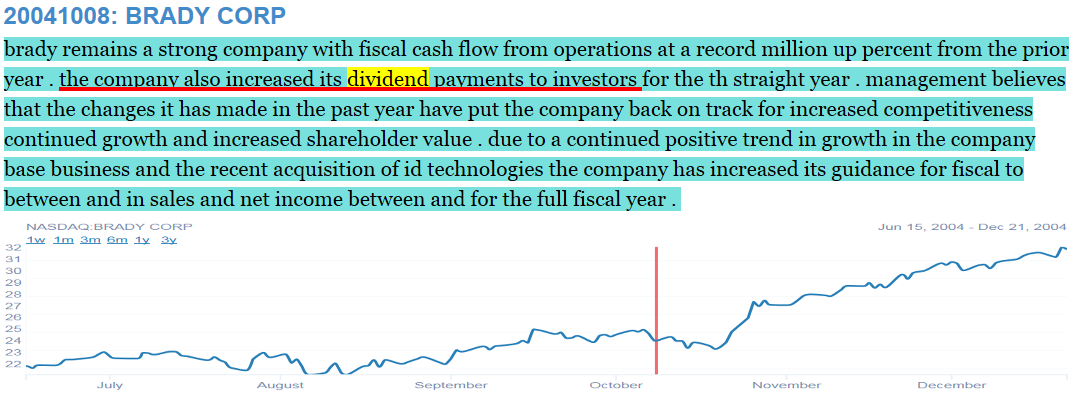
\includegraphics[height=1.65in, width=3.5in]{fig/dividend_positive.png}
\caption{A low-risk word
in a low-risk sentence} \label{fig:dividend_lowrisksentence}
\end{figure}

\begin{figure}[tbh]
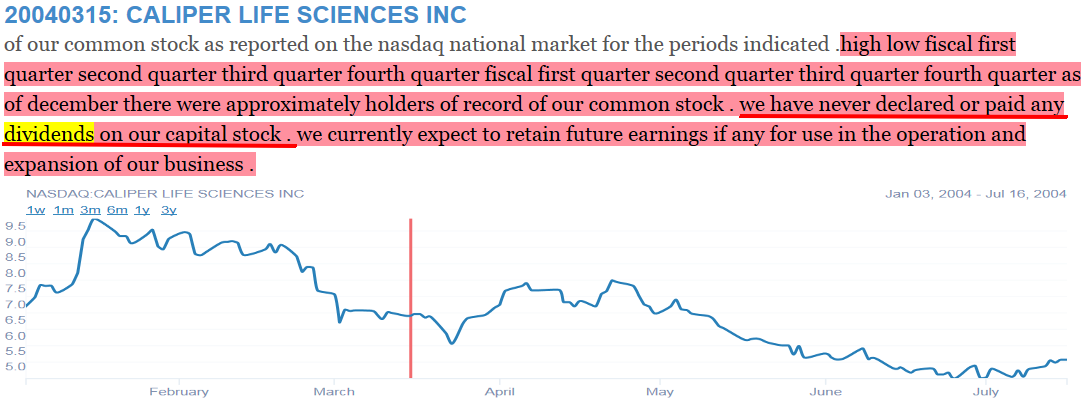
\includegraphics[height=1.65in, width=3.5in]{fig/dividend_negative.png}
\caption{A low-risk word
in a high-risk sentence}\label{fig:dividend_highrisksentence}
\end{figure}
    Here we showcase some interesting cases to demonstrate the need to conduct sentence-level analysis on finance textual information and the usability of the proposed system.
    The word ``dividend'' displayed as follows is a notable example.
    According to financial literature such as~\cite{denis2008firms}, dividend is empirically treated as a low-risk word because companies with the propensity to pay dividends are assumed to be profitable ones.
    Figure~\ref{fig:dividend_lowrisksentence} shows Brady Corp.'s stock prices trend upward after the announcement of its year 2004 financial report stating that
    ``the company also increased its dividend payments to investors \ldots.'' However, Figure~\ref{fig:dividend_highrisksentence} exhibits an opposite case from the sentence-level point of view,
    because another company, Caliper Life Science Inc.\ states that ``we have never declared or paid any dividends on our capital stock'' in its year 2004 report.
    The high-risk word ``deficit'' is another notable example.
    This word is sometimes utilized to reveal positive signals like ``reducing the company working capital deficit and increase liquidity $\ldots$''\footnote{For example, see Mallon Resources Corp.'s annual report for 1996.}
    or usual negative ones like ``the gross deficit incurred resulted from costs of products $\ldots$.''
    %Several similar cases can also be founded via the proposed RiskFinder system.
    %For example, from the sentence-level analysis point of view, the low-risk word ``profit'' (discovered in the study of~\cite{tsai2017risk}) may refer to either ``increase in gross profits'' or ``reduction in gross profits.''
    %the high-risk word ``deficit'' sometimes reveals positive signals such as ``reducing the company working capital deficit and increase liquidity $\ldots$''\footnote{For example, see Mallon Resources Corp.'s annual report for 1996.}
    %or the usual negative ones like ``the gross deficit incurred resulted from costs of products $\ldots$.''

\section{Conclusions}\label{sec:conclusion}
    In this paper we introduce RiskFinder, a web-based information system that broadens the textual analysis of financial reports from the word level to the sentence level. This extension is essential especially for the analysis of financial keywords because most of these words are context-sensitive. Built on financial reports in the 10-K Corpus with a set of labeled sentences about financial risk, this proposed system applies two sentence embedding techniques --- FastText and Siamese-CBOW --- to automatically classify the risk-related sentences in those reports as being positively, negatively or insignificantly related to financial risk. For comparison purposes, the system even displays the time-aligned relevant quantitative information to visualize the financial risk associated with the announcement of each report. This system greatly facilitates case studies in the finance field for scholars and can be of great help for practitioners in capturing meaningful insight within large amounts of textual information in finance from the sentence-level point of view. The system is now online available at~\url{https://cfda.csie.org/RiskFinder/}.

    This work is a preliminary study, the purpose of which is to demonstrate the importance of sentence-level analysis and the integration of soft and hard information in finance. Therefore, in the future, we will continue to extend the system, with an emphasis on incorporating more state-of-the-art learning algorithms or developing new algorithms to better detect risk-related sentences.

\bibliographystyle{IEEEtran}
\bibliography{paper}
\end{document}
